\chapter{Background}
\section{Category Theory}
\subsection{Categories}

A category formally is a collection of objects and morphisms that follow a composition law \cite{context}. \todo{Expand on this. Should I give an actual definition of an abstract category? I probably should}

While this definition is very abstract, it is useful in describing a lot of things \todo{find a better word} in mathematics.
Some of the most useful categories for application are \emph{concrete} categories, which practically are categories whose objects spaces with some form of structure and morphisms are structure preserving mappings between them.


\missingfigure{Make a diagram to represent a few objects/morphisms in $\Set$.}
\missingfigure{Make a diagram to represent a few objects/morphisms in $\FinVect$. Make it look congruent to $\Set$.}

An example is shown in $\Set$ and $\FinVect$.
The category $\Set$ has sets as its objects, and its morphisms are functions.
The category $\FinVect$ has as its objects finite dimensional vector spaces over the real numbers as their bed of scalars, and its morphisms are linear transformations\footnote{These transformations can be represented by a matrix, but only if a basis is provided for both domain and codomain. We should not automatically assume a vector space has a canonical basis that's best for the job!}.
Note that $\FinVect$ is just a subcategory\footnote{I won't define it, but I hope it's not hard to imagine what a subcategory is. Closure under composition is the main requirement.} of $\Set$. This is talked about in more detail in books.\todo{Specify}

This view is different from a set theoretic approach to fields in mathematics.
For instance, the set theoretic approach to linear algebra would define a vector space as a set with a certain algebraic structure, and a linear transformation as a function preserving that structure in a certain way.
A categorical approach would instead define the category of vector spaces as a collection of objects (the vector spaces) and of morphisms\footnote{and of functors. more on that later}, and would specify how morphisms behave in composition.
This approach is described as "context rich and content poor"\todo{cite youtube video}
\todo[inline]{Finish this paragraph. Element poor, but we can get around that, and the language is unified to describe similar phenomena in different fields, blah blah blah}

\todo[inline]{Talk about functional programming}
\todo[inline]{Talk about how Markov categories are cats with markov kernels}

\subsection{Functors}
\subsubsection{Example Functors}
\subsection{Monoidal Functors}
\subsection{Natural Transformations}
\subsection{Monads}
\subsection{Kleisli Categories}

\section{Markov Categories}

\subsection{Example: Set}
\subsection{Kleisli Categories}

\section{String Diagrams}

String diagrams are very similar to the signal flow diagrams or block diagrams found in control systems.
Others (\cite{baez2015control}, \cite{fong2016thesis}, \cite{fong2016dynamicalsystems}) have drawn the connections between string diagrams and various diagrams in systems engineering including block diagrams for dynamical systems.

There are often two interpretations in block diagrams:
In what I will call the temporal interpretation, the state of a diagram can be seen as changing over time, where the states are carried by the wires from block to block. The blocks represent state transformations, which are applied continuously to their inputs to generate changing outputs.
There may be blocks which carry their own internal state, such as integrators, that keep track of quantities over time to affect their output\todo{This sentence sucks.}

In what I'll call the signal flow interpretation, a time-varying signal is seen as a single entity, and the blocks represent signals in transformation space. This interpretation allows for a more functional analysis type approach to control design.

String diagrams look quite similar to block diagrams, but their interpretation is very different.
Blocks are still seen as transformations, but they then become the primary point of interest instead of the "signals" themselves.
The wires do not represent signals, but rather state spaces.
Whenever a wire splits, or disappears, or loops around, that becomes interpreted as a special transformation itself.
With this interpretation, a string diagram simply becomes a tool to draw out complicated compositions of transformations, or morphisms in a symmetric monoidal category.

\subsection{Explanation of String Diagrams}

\subsection{Translating String Diagrams into Kernel Compositions}
String diagrams allow us to write complicated equations with a single picture that can then be systematically translated back into equations for computation.
These pictures are often much clearer to interpret, and easier to memorize as they can be puzzle pieced together.
Interpreting them is straightforward: Take the example problem of finding the conditional of a kernel with respect to part of its output.
This problem statement carries with it the nuance of the complexity in finding conditionals, unlike the simple measure theoretic definition.

Given $f:A\rightarrow X\otimes Y$, find $f_X : X\otimes A \rightarrow Y$ such that the equation in Figure \ref{fig:conditional} holds.

\begin{figure}[htb]
	\centering
	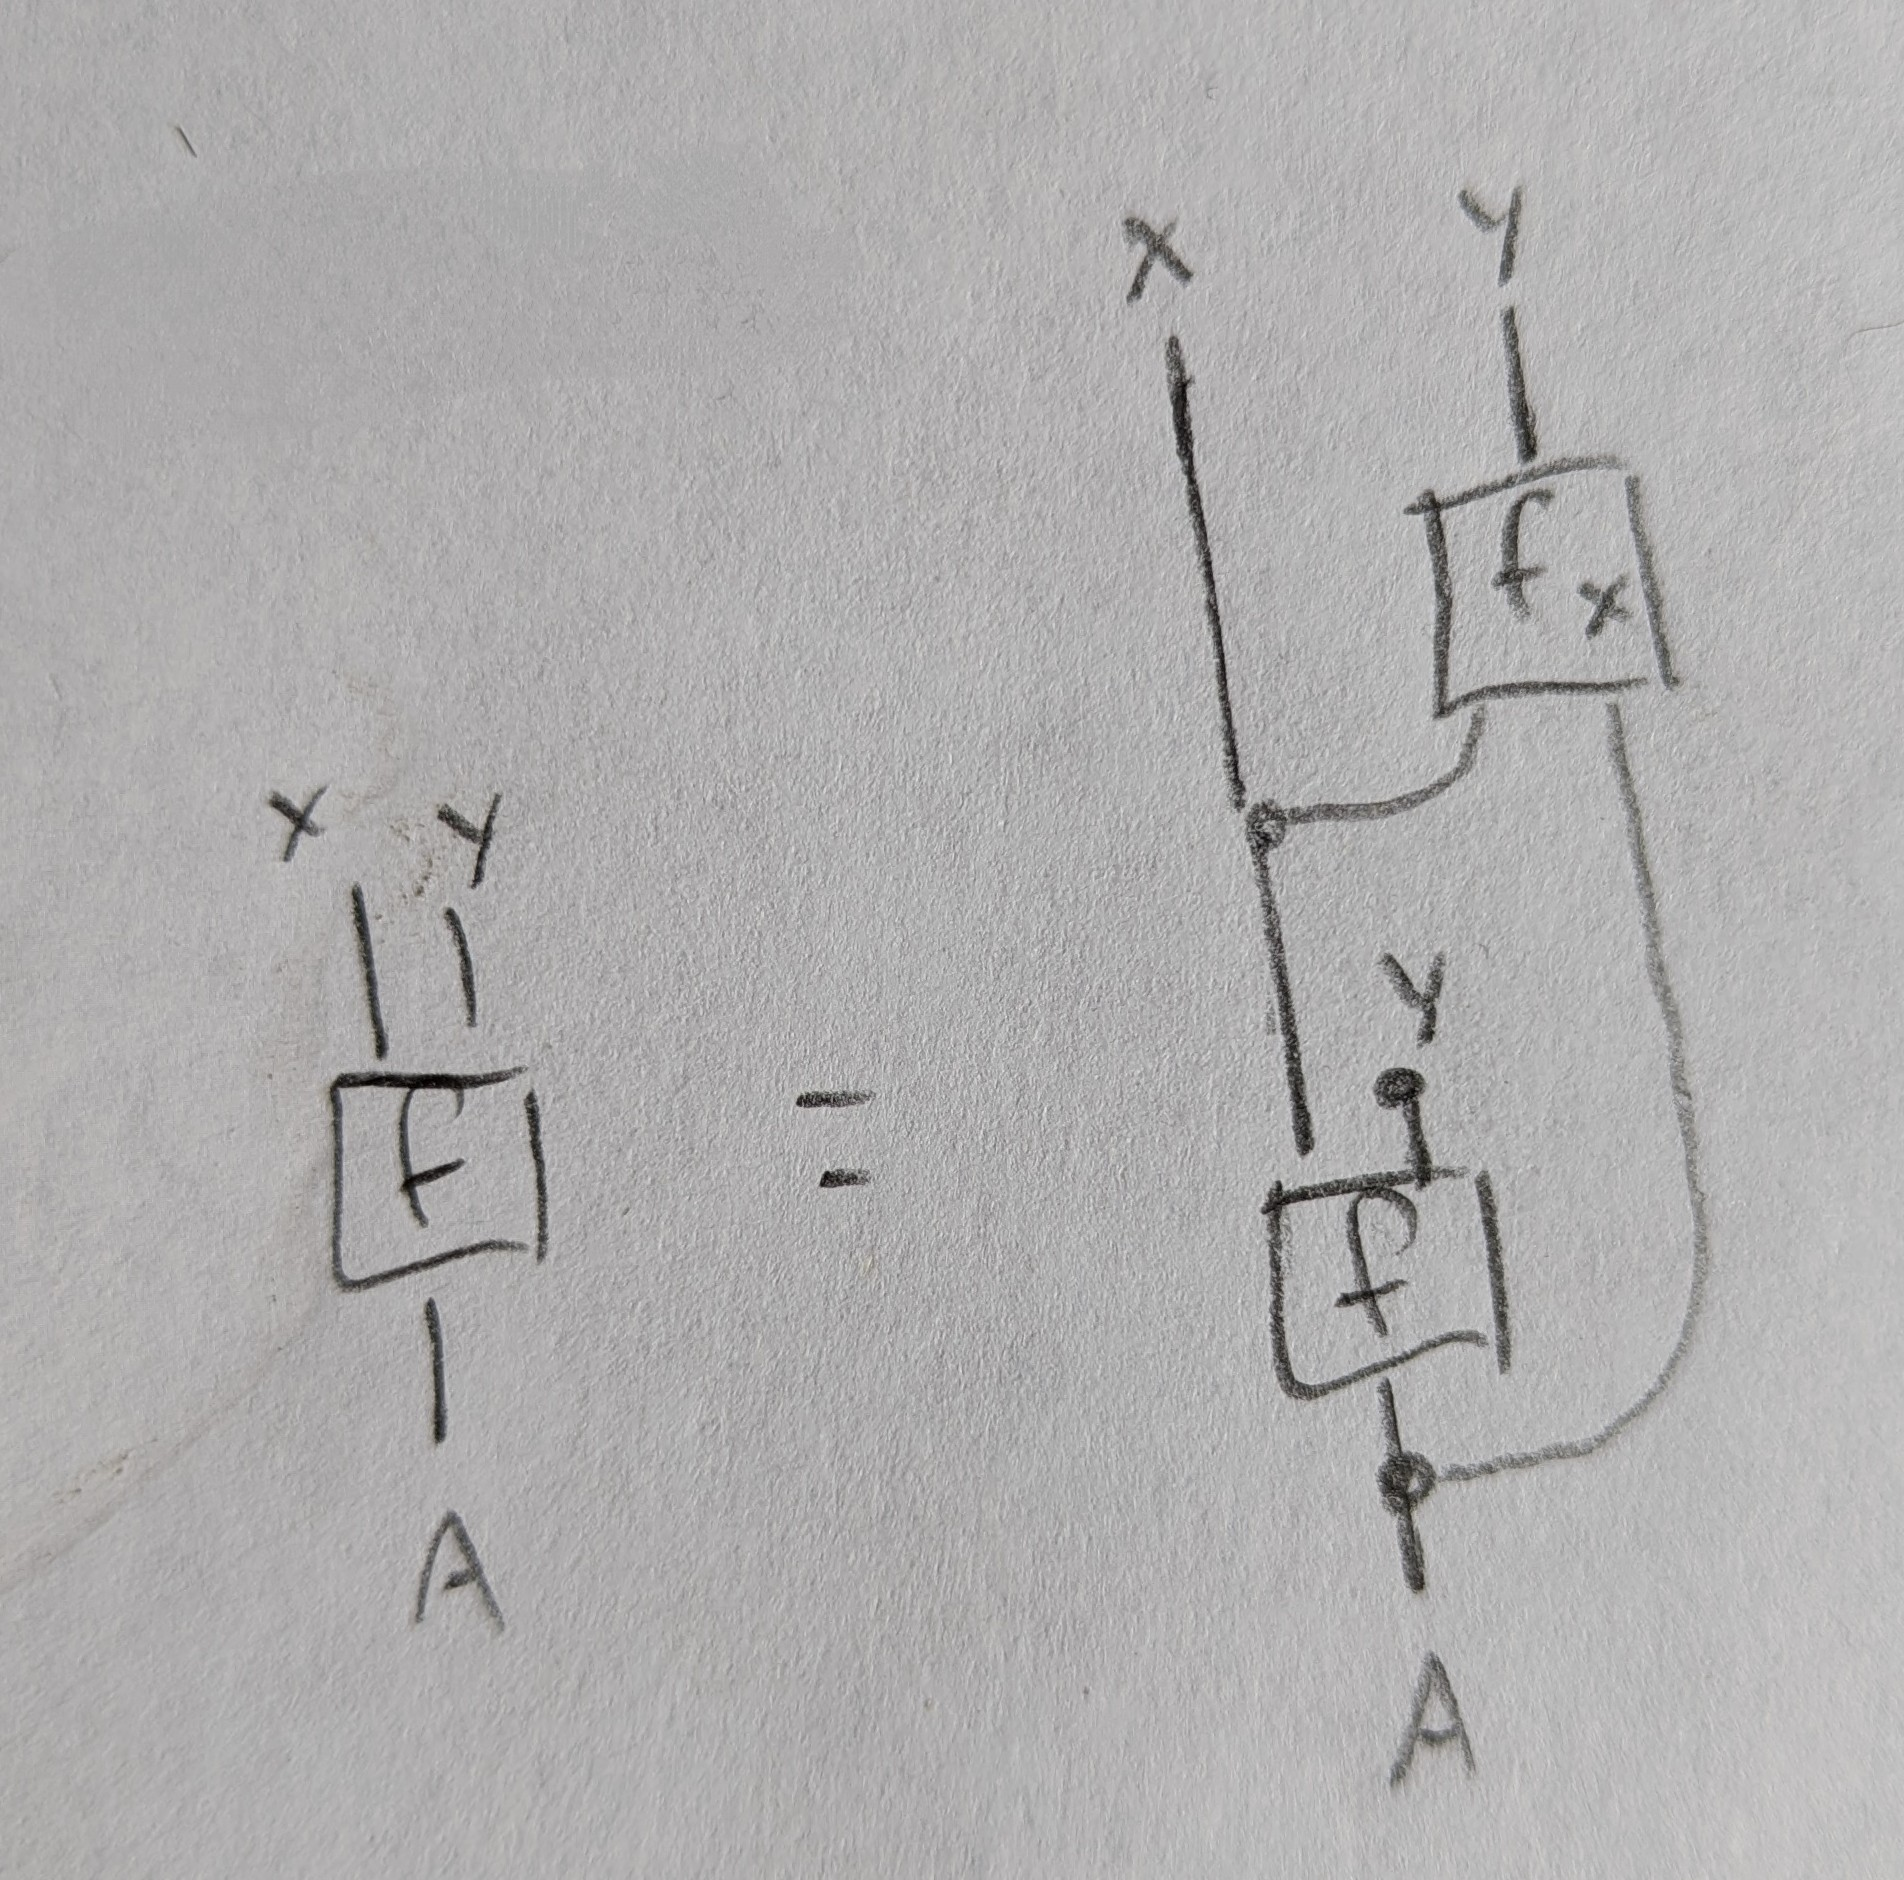
\includegraphics[width=0.5\textwidth]{conditional}
	\caption{The string diagram equation for the definition of conditioning.}
	\label{fig:conditional}
\end{figure}

\begin{figure}[htb]
	\centering
	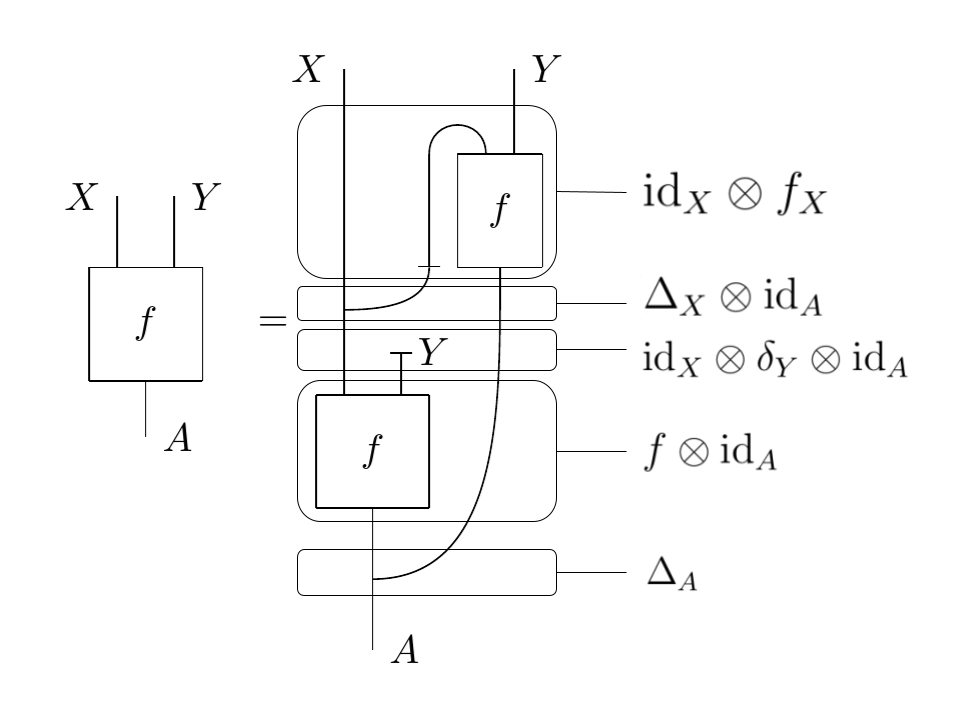
\includegraphics[width=0.5\textwidth]{conditional-compositions}
	\caption{The conditional equation is read like so. This corresponds to Equation \ref{eq:conditional-compositions}.}
	\label{fig:conditional-compositions}
\end{figure}

\begin{figure}[htb]
	\centering
	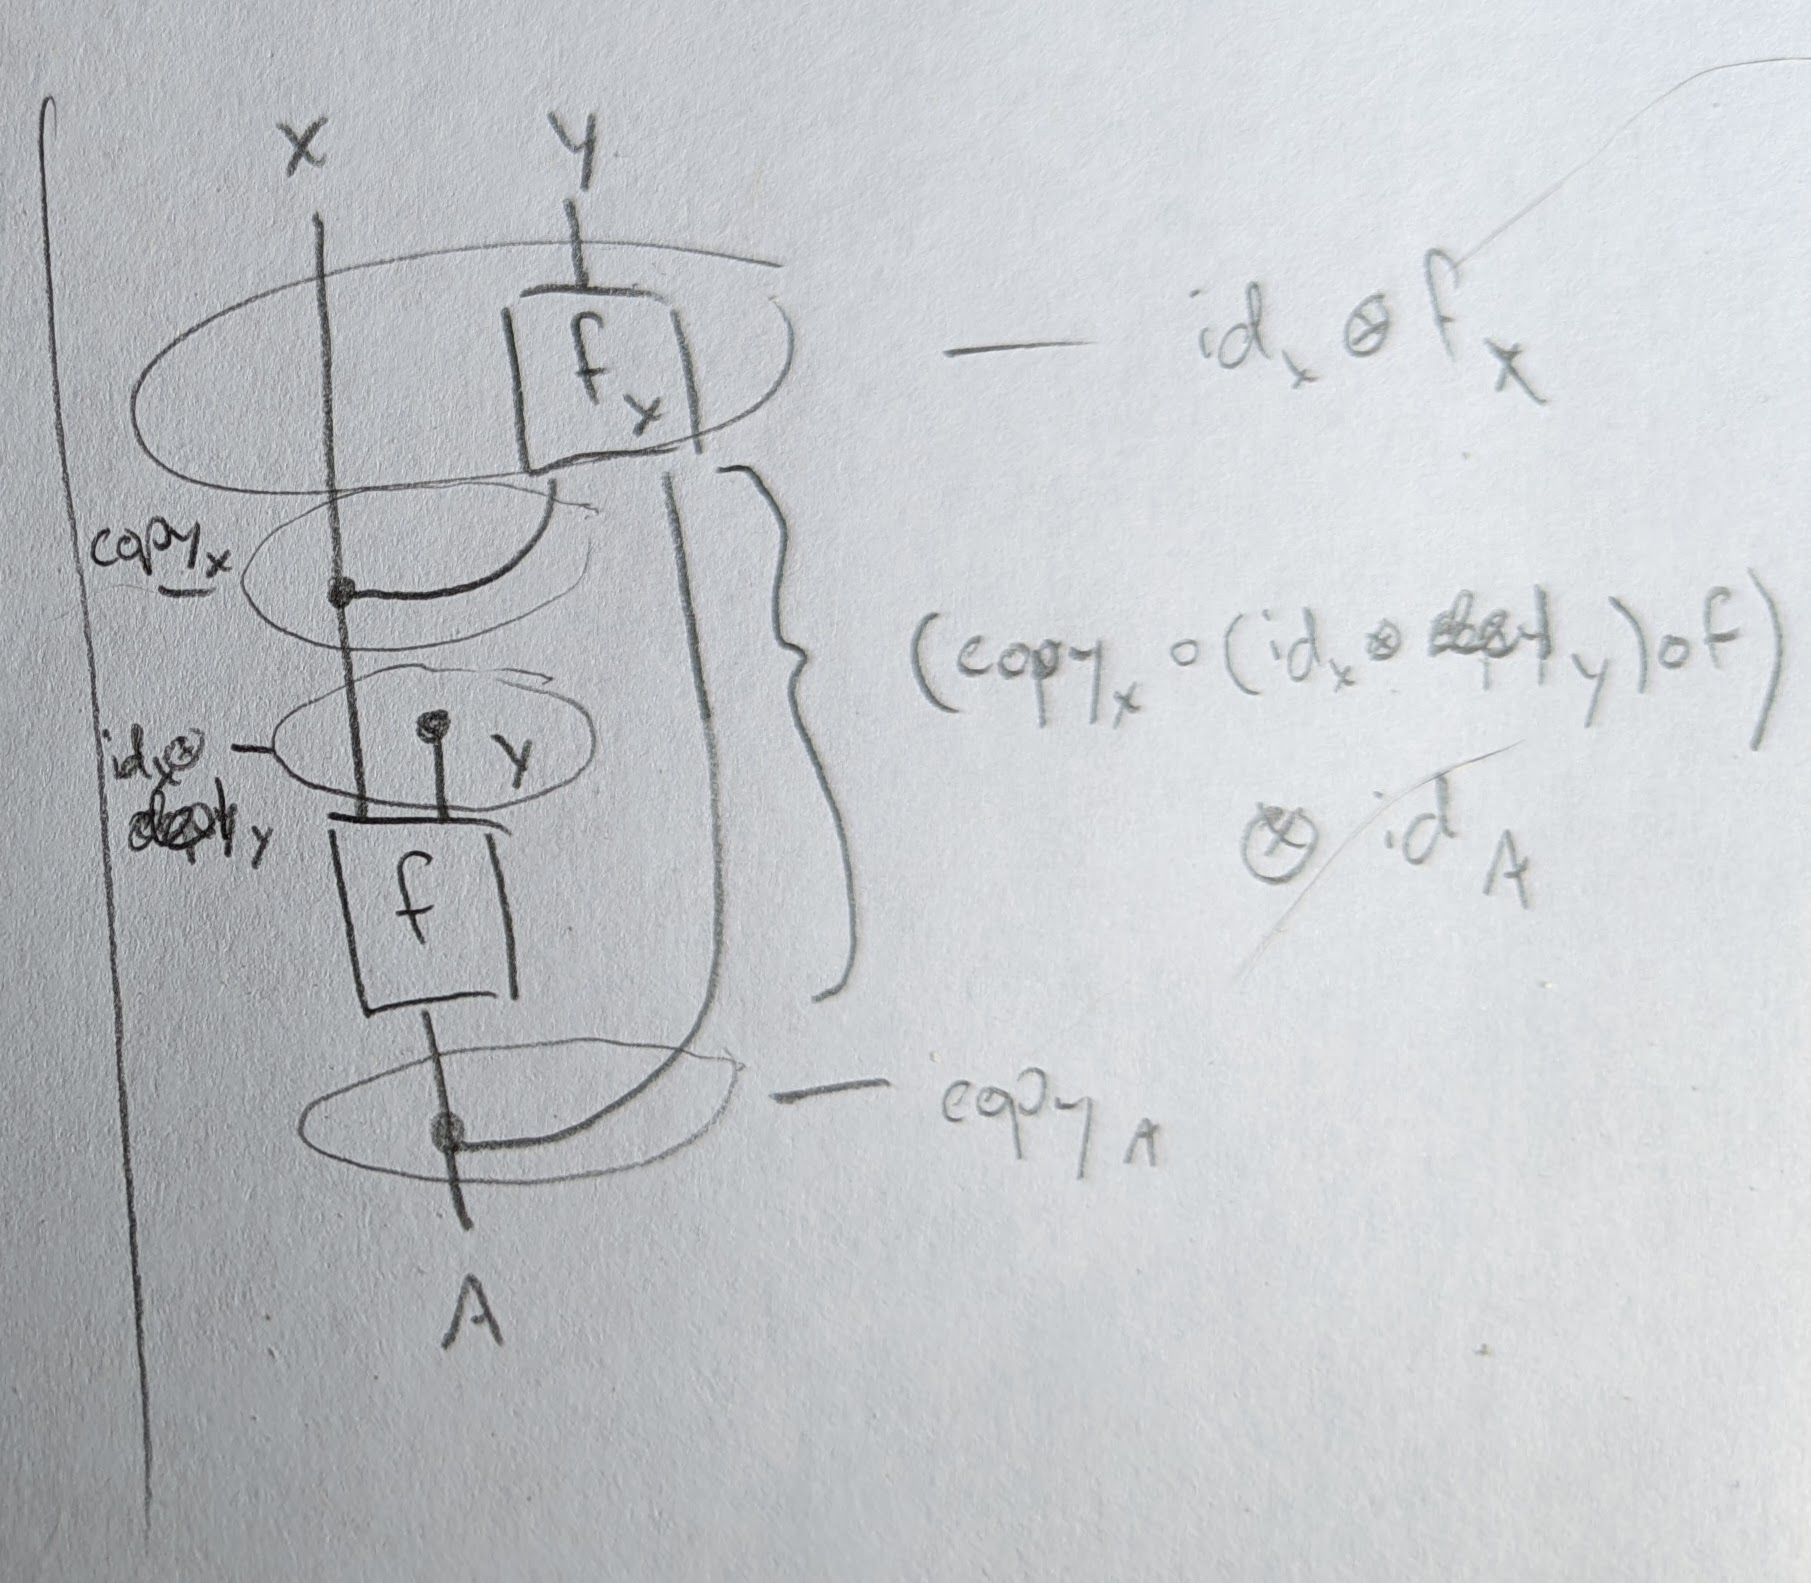
\includegraphics[width=0.5\textwidth]{conditional-parallel-compositions}
	\caption{The conditional equation can also be read this way. This corresponds to Equation \ref{eq:conditional-parallel-compositions}.}
	\label{fig:conditional-parallel-compositions}
\end{figure}

\begin{equation}
\label{eq:conditional-compositions}
f = (\counit_X \otimes f) \circ (\comul_X \otimes \id_A)
\circ (\id_X \otimes \counit_Y \otimes \id_A) \circ (f \otimes \id_A) \circ \comul_A
\end{equation}

\begin{equation}
\label{eq:conditional-parallel-compositions}
f = (\id_x \otimes f_x) \circ \left[\left(\comul_x \circ (\id_x\otimes \counit_Y) \circ f\right) \otimes \id_A\right] \circ \comul_A
\end{equation}

** Explain notation. Every operator you are using in these equations should be explained and formally introduced. **

\section{Bar Notation}
\subsection{Explanation of Bar Notation}
\subsection{Translating Bar Notation into String Diagrams}

\chapter{Common Representations of Information Recast into the Language of Markov Categories}
\section{Discrete Probability}
\section{Gaussian Probability}
\section{Gaussian Mixtures: A Composition of Discrete and Gaussian Probability}
\section{Unscented Transform}

\chapter{Programming with Markov Categories}
\section{Making Datatypes}
\subsection{Gaussian}
\subsection{Unscented}
\subsection{Gaussian Mixtures}

\section{Synthetic Algorithms Used in Estimation and Control}
\subsection{Filtering}
\subsection{History Space}

